%!TEX root = ../../report.tex

\subsection{Undiscovered City} % (fold)
\label{sub:undiscovered_city}

In the ``Real-time Procedural Generation of ‘Pseudo Infinite’ Cities" paper, from Stefan Greuter et al. presented a system that generates in Real-time pseudo infinite virtual cities which can be interactively explored from a first person perspective. ``All geometrical components of the city are generated as they are encountered by the user." As shown in the following image only the part of city that is inside the viewing range is generate.

\begin{figure}[htbp]
	\centering
	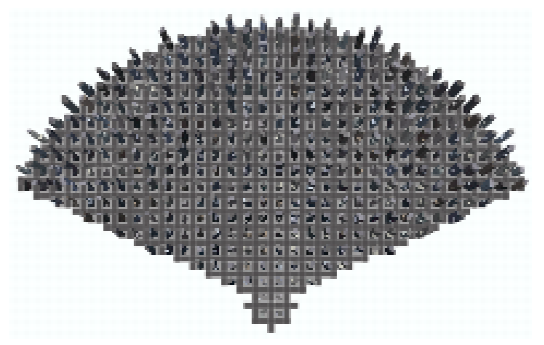
\includegraphics[width=0.85\textwidth]{img/Real-Time-procedural-generation/viewing-range.png}
	\caption{buildings}
	\label{fig:label}
\end{figure}

\subsubsection{Road Network} % (fold)
\label{ssub:road_network}

The system uses a 2D grid that divide the terrain into square cells. The cells represent proxies for the content that will be procedurally generated. Before the content of each cell is generated, the potential visibility of it is tested, and after that, only the visible cells are filled with content.

After that the roads are created in a uniform grid pattern. This grid does not feel very natural, and in the continuation of the work, this system evolved into a more realistic one with the join of some of the grids to create a less uniform distribution of the buildings.

% subsubsection road_network (end)

\subsubsection{Buildings} % (fold)
\label{ssub:buildings}


To compute the form and appearance of each building, it is used a ``single 32 bit pseudo random number generator seed. The random sequence determines building properties such as width, height and number of floors."
Similar sequences of number result in similar buildings. To avoid that, it is used a a hash function to convert each cell position into a seed.

To generate a building is first is generated a floor plan. To do so, it's randomly selected and merged a set of regular polygons and rectangles, then this is extruded. This is an iterative process, that creates sections from the top to the bottom, by adding more shapes to the the initial shape and extruding as shown in the Figure~\ref{fig:buildings}.

\begin{figure}[htbp]
	\centering
	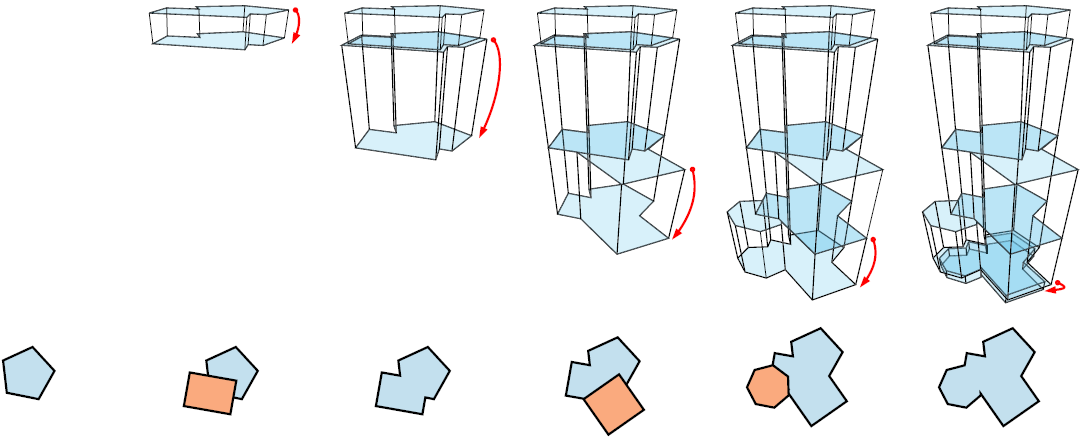
\includegraphics[width=0.85\textwidth]{img/Real-Time-procedural-generation/Building-Generation.png}
	\caption{buildings}
	\label{fig:label}
\end{figure}


Starting from the left, first there is a simple polygon, that is merged with a rectangle and after extrusion, forms the first block that will be the top of the building. After that, another extrusion is made to generate the next block. After that is merged a rectangle to the floor shape and generated a new block and so on.
% subsubsection buildings (end)

% subsection undiscovered_city (end)